\documentclass[1p]{elsarticle_modified}
%\bibliographystyle{elsarticle-num}

%\usepackage[colorlinks]{hyperref}
%\usepackage{abbrmath_seonhwa} %\Abb, \Ascr, \Acal ,\Abf, \Afrak
\usepackage{amsfonts}
\usepackage{amssymb}
\usepackage{amsmath}
\usepackage{amsthm}
\usepackage{scalefnt}
\usepackage{amsbsy}
\usepackage{kotex}
\usepackage{caption}
\usepackage{subfig}
\usepackage{color}
\usepackage{graphicx}
\usepackage{xcolor} %% white, black, red, green, blue, cyan, magenta, yellow
\usepackage{float}
\usepackage{setspace}
\usepackage{hyperref}

\usepackage{tikz}
\usetikzlibrary{arrows}

\usepackage{multirow}
\usepackage{array} % fixed length table
\usepackage{hhline}

%%%%%%%%%%%%%%%%%%%%%
\makeatletter
\renewcommand*\env@matrix[1][\arraystretch]{%
	\edef\arraystretch{#1}%
	\hskip -\arraycolsep
	\let\@ifnextchar\new@ifnextchar
	\array{*\c@MaxMatrixCols c}}
\makeatother %https://tex.stackexchange.com/questions/14071/how-can-i-increase-the-line-spacing-in-a-matrix
%%%%%%%%%%%%%%%

\usepackage[normalem]{ulem}

\newcommand{\msout}[1]{\ifmmode\text{\sout{\ensuremath{#1}}}\else\sout{#1}\fi}
%SOURCE: \msout is \stkout macro in https://tex.stackexchange.com/questions/20609/strikeout-in-math-mode

\newcommand{\cancel}[1]{
	\ifmmode
	{\color{red}\msout{#1}}
	\else
	{\color{red}\sout{#1}}
	\fi
}

\newcommand{\add}[1]{
	{\color{blue}\uwave{#1}}
}

\newcommand{\replace}[2]{
	\ifmmode
	{\color{red}\msout{#1}}{\color{blue}\uwave{#2}}
	\else
	{\color{red}\sout{#1}}{\color{blue}\uwave{#2}}
	\fi
}

\newcommand{\Sol}{\mathcal{S}} %segment
\newcommand{\D}{D} %diagram
\newcommand{\A}{\mathcal{A}} %arc


%%%%%%%%%%%%%%%%%%%%%%%%%%%%%5 test

\def\sl{\operatorname{\textup{SL}}(2,\Cbb)}
\def\psl{\operatorname{\textup{PSL}}(2,\Cbb)}
\def\quan{\mkern 1mu \triangleright \mkern 1mu}

\theoremstyle{definition}
\newtheorem{thm}{Theorem}[section]
\newtheorem{prop}[thm]{Proposition}
\newtheorem{lem}[thm]{Lemma}
\newtheorem{ques}[thm]{Question}
\newtheorem{cor}[thm]{Corollary}
\newtheorem{defn}[thm]{Definition}
\newtheorem{exam}[thm]{Example}
\newtheorem{rmk}[thm]{Remark}
\newtheorem{alg}[thm]{Algorithm}

\newcommand{\I}{\sqrt{-1}}
\begin{document}

%\begin{frontmatter}
%
%\title{Boundary parabolic representations of knots up to 8 crossings}
%
%%% Group authors per affiliation:
%\author{Yunhi Cho} 
%\address{Department of Mathematics, University of Seoul, Seoul, Korea}
%\ead{yhcho@uos.ac.kr}
%
%
%\author{Seonhwa Kim} %\fnref{s_kim}}
%\address{Center for Geometry and Physics, Institute for Basic Science, Pohang, 37673, Korea}
%\ead{ryeona17@ibs.re.kr}
%
%\author{Hyuk Kim}
%\address{Department of Mathematical Sciences, Seoul National University, Seoul 08826, Korea}
%\ead{hyukkim@snu.ac.kr}
%
%\author{Seokbeom Yoon}
%\address{Department of Mathematical Sciences, Seoul National University, Seoul, 08826,  Korea}
%\ead{sbyoon15@snu.ac.kr}
%
%\begin{abstract}
%We find all boundary parabolic representation of knots up to 8 crossings.
%
%\end{abstract}
%\begin{keyword}
%    \MSC[2010] 57M25 
%\end{keyword}
%
%\end{frontmatter}

%\linenumbers
%\tableofcontents
%
\newcommand\colored[1]{\textcolor{white}{\rule[-0.35ex]{0.8em}{1.4ex}}\kern-0.8em\color{red} #1}%
%\newcommand\colored[1]{\textcolor{white}{ #1}\kern-2.17ex	\textcolor{white}{ #1}\kern-1.81ex	\textcolor{white}{ #1}\kern-2.15ex\color{red}#1	}

{\Large $\underline{12n_{0141}~(K12n_{0141})}$}

\setlength{\tabcolsep}{10pt}
\renewcommand{\arraystretch}{1.6}
\vspace{1cm}\begin{tabular}{m{100pt}>{\centering\arraybackslash}m{274pt}}
\multirow{5}{120pt}{
	\centering
	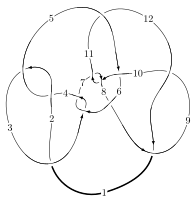
\includegraphics[width=112pt]{../../../GIT/diagram.site/Diagrams/png/2230_12n_0141.png}\\
\ \ \ A knot diagram\footnotemark}&
\allowdisplaybreaks
\textbf{Linearized knot diagam} \\
\cline{2-2}
 &
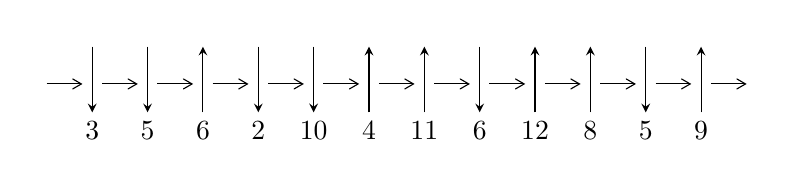
\begin{tikzpicture}[x=20pt, y=17pt]
	% nodes
	\node (C0) at (0, 0) {};
	\node (C1) at (1, 0) {};
	\node (C1U) at (1, +1) {};
	\node (C1D) at (1, -1) {3};

	\node (C2) at (2, 0) {};
	\node (C2U) at (2, +1) {};
	\node (C2D) at (2, -1) {5};

	\node (C3) at (3, 0) {};
	\node (C3U) at (3, +1) {};
	\node (C3D) at (3, -1) {6};

	\node (C4) at (4, 0) {};
	\node (C4U) at (4, +1) {};
	\node (C4D) at (4, -1) {2};

	\node (C5) at (5, 0) {};
	\node (C5U) at (5, +1) {};
	\node (C5D) at (5, -1) {10};

	\node (C6) at (6, 0) {};
	\node (C6U) at (6, +1) {};
	\node (C6D) at (6, -1) {4};

	\node (C7) at (7, 0) {};
	\node (C7U) at (7, +1) {};
	\node (C7D) at (7, -1) {11};

	\node (C8) at (8, 0) {};
	\node (C8U) at (8, +1) {};
	\node (C8D) at (8, -1) {6};

	\node (C9) at (9, 0) {};
	\node (C9U) at (9, +1) {};
	\node (C9D) at (9, -1) {12};

	\node (C10) at (10, 0) {};
	\node (C10U) at (10, +1) {};
	\node (C10D) at (10, -1) {8};

	\node (C11) at (11, 0) {};
	\node (C11U) at (11, +1) {};
	\node (C11D) at (11, -1) {5};

	\node (C12) at (12, 0) {};
	\node (C12U) at (12, +1) {};
	\node (C12D) at (12, -1) {9};
	\node (C13) at (13, 0) {};

	% arrows
	\draw[->,>={angle 60}]
	(C0) edge (C1) (C1) edge (C2) (C2) edge (C3) (C3) edge (C4) (C4) edge (C5) (C5) edge (C6) (C6) edge (C7) (C7) edge (C8) (C8) edge (C9) (C9) edge (C10) (C10) edge (C11) (C11) edge (C12) (C12) edge (C13) ;	\draw[->,>=stealth]
	(C1U) edge (C1D) (C2U) edge (C2D) (C3D) edge (C3U) (C4U) edge (C4D) (C5U) edge (C5D) (C6D) edge (C6U) (C7D) edge (C7U) (C8U) edge (C8D) (C9D) edge (C9U) (C10D) edge (C10U) (C11U) edge (C11D) (C12D) edge (C12U) ;
	\end{tikzpicture} \\
\hhline{~~} \\& 
\textbf{Solving Sequence} \\ \cline{2-2} 
 &
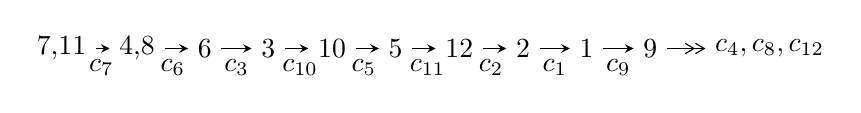
\begin{tikzpicture}[x=23pt, y=7pt]
	% node
	\node (A0) at (-1/8, 0) {7,11};
	\node (A1) at (17/16, 0) {4,8};
	\node (A2) at (17/8, 0) {6};
	\node (A3) at (25/8, 0) {3};
	\node (A4) at (33/8, 0) {10};
	\node (A5) at (41/8, 0) {5};
	\node (A6) at (49/8, 0) {12};
	\node (A7) at (57/8, 0) {2};
	\node (A8) at (65/8, 0) {1};
	\node (A9) at (73/8, 0) {9};
	\node (C1) at (1/2, -1) {$c_{7}$};
	\node (C2) at (13/8, -1) {$c_{6}$};
	\node (C3) at (21/8, -1) {$c_{3}$};
	\node (C4) at (29/8, -1) {$c_{10}$};
	\node (C5) at (37/8, -1) {$c_{5}$};
	\node (C6) at (45/8, -1) {$c_{11}$};
	\node (C7) at (53/8, -1) {$c_{2}$};
	\node (C8) at (61/8, -1) {$c_{1}$};
	\node (C9) at (69/8, -1) {$c_{9}$};
	\node (A10) at (11, 0) {$c_{4},c_{8},c_{12}$};

	% edge
	\draw[->,>=stealth]	
	(A0) edge (A1) (A1) edge (A2) (A2) edge (A3) (A3) edge (A4) (A4) edge (A5) (A5) edge (A6) (A6) edge (A7) (A7) edge (A8) (A8) edge (A9) ;
	\draw[->>,>={angle 60}]	
	(A9) edge (A10);
\end{tikzpicture} \\ 

\end{tabular} \\

\footnotetext{
The image of knot diagram is generated by the software ``\textbf{Draw programme}" developed by Andrew Bartholomew(\url{http://www.layer8.co.uk/maths/draw/index.htm\#Running-draw}), where we modified some parts for our purpose(\url{https://github.com/CATsTAILs/LinksPainter}).
}\phantom \\ \newline 
\centering \textbf{Ideals for irreducible components\footnotemark of $X_{\text{par}}$} 
 
\begin{align*}
I^u_{1}&=\langle 
-6686875043 u^{25}-624104415 u^{24}+\cdots+13435529728 b+3806288503,\\
\phantom{I^u_{1}}&\phantom{= \langle  }79755561391 u^{25}+46013804251 u^{24}+\cdots+214968475648 a-231933695795,\\
\phantom{I^u_{1}}&\phantom{= \langle  }u^{26}+2 u^{24}+\cdots- u+1\rangle \\
I^u_{2}&=\langle 
-6.09745\times10^{15} u^{23}+2.23561\times10^{15} u^{22}+\cdots+4.70830\times10^{16} b-9.49470\times10^{16},\\
\phantom{I^u_{2}}&\phantom{= \langle  }3.77245\times10^{16} u^{23}-4.36637\times10^{15} u^{22}+\cdots+1.14344\times10^{17} a+1.28843\times10^{18},\;u^{24}-2 u^{23}+\cdots+20 u+17\rangle \\
I^u_{3}&=\langle 
b,\;- u^3- u^2+4 a+2 u-3,\;u^4+u^2+u+1\rangle \\
I^u_{4}&=\langle 
13362 a^5 u-25075 a^4 u+\cdots+39143 a+74777,\\
\phantom{I^u_{4}}&\phantom{= \langle  }a^6-5 a^5 u-5 a^5+14 a^4 u+2 a^3 u+9 a^3-14 a^2 u+10 a^2-5 a u-13 a+3 u,\;u^2+1\rangle \\
I^u_{5}&=\langle 
b,\;- u^3+a- u+1,\;u^6- u^5+2 u^4-2 u^3+2 u^2-2 u+1\rangle \\
\\
\end{align*}
\raggedright * 5 irreducible components of $\dim_{\mathbb{C}}=0$, with total 72 representations.\\
\footnotetext{All coefficients of polynomials are rational numbers. But the coefficients are sometimes approximated in decimal forms when there is not enough margin.}
\newpage
\renewcommand{\arraystretch}{1}
\centering \section*{I. $I^u_{1}= \langle -6.69\times10^{9} u^{25}-6.24\times10^{8} u^{24}+\cdots+1.34\times10^{10} b+3.81\times10^{9},\;7.98\times10^{10} u^{25}+4.60\times10^{10} u^{24}+\cdots+2.15\times10^{11} a-2.32\times10^{11},\;u^{26}+2 u^{24}+\cdots- u+1 \rangle$}
\flushleft \textbf{(i) Arc colorings}\\
\begin{tabular}{m{7pt} m{180pt} m{7pt} m{180pt} }
\flushright $a_{7}=$&$\begin{pmatrix}1\\0\end{pmatrix}$ \\
\flushright $a_{11}=$&$\begin{pmatrix}0\\u\end{pmatrix}$ \\
\flushright $a_{4}=$&$\begin{pmatrix}-0.371010 u^{25}-0.214049 u^{24}+\cdots-2.37389 u+1.07892\\0.497701 u^{25}+0.0464518 u^{24}+\cdots-0.303652 u-0.283300\end{pmatrix}$ \\
\flushright $a_{8}=$&$\begin{pmatrix}1\\- u^2\end{pmatrix}$ \\
\flushright $a_{6}=$&$\begin{pmatrix}0.786727 u^{25}+0.355240 u^{24}+\cdots+0.268947 u+0.181402\\-0.281655 u^{25}+0.162782 u^{24}+\cdots-0.150036 u+1.19156\end{pmatrix}$ \\
\flushright $a_{3}=$&$\begin{pmatrix}-0.0563150 u^{25}-0.379621 u^{24}+\cdots-1.27287 u-1.11514\\0.478616 u^{25}-0.0163741 u^{24}+\cdots+1.75358 u-0.0264586\end{pmatrix}$ \\
\flushright $a_{10}=$&$\begin{pmatrix}- u\\u^3+u\end{pmatrix}$ \\
\flushright $a_{5}=$&$\begin{pmatrix}0.836319 u^{25}+0.321913 u^{24}+\cdots+0.240330 u-0.254796\\-0.290547 u^{25}+0.204134 u^{24}+\cdots-0.0385003 u+1.59443\end{pmatrix}$ \\
\flushright $a_{12}=$&$\begin{pmatrix}-0.00390625 u^{25}-0.00390625 u^{24}+\cdots-2 u-0.996094\\0.00781250 u^{25}+0.00781250 u^{24}+\cdots+2 u-0.00781250\end{pmatrix}$ \\
\flushright $a_{2}=$&$\begin{pmatrix}-0.977915 u^{25}-0.402299 u^{24}+\cdots-2.88010 u+0.873808\\0.278382 u^{25}-0.0788085 u^{24}+\cdots-1.17498 u-1.03877\end{pmatrix}$ \\
\flushright $a_{1}=$&$\begin{pmatrix}0.00781250 u^{25}+0.00781250 u^{24}+\cdots+2 u+0.992188\\-\frac{1}{64} u^{25}-\frac{1}{64} u^{24}+\cdots-2 u+\frac{1}{64}\end{pmatrix}$ \\
\flushright $a_{9}=$&$\begin{pmatrix}-0.00390625 u^{25}-0.00390625 u^{24}+\cdots-2 u+0.00390625\\\frac{1}{128} u^{25}+\frac{1}{128} u^{24}+\cdots+u-\frac{1}{128}\end{pmatrix}$\\&\end{tabular}
\flushleft \textbf{(ii) Obstruction class $= -1$}\\~\\
\flushleft \textbf{(iii) Cusp Shapes $= \frac{2427750693445}{859873902592} u^{25}-\frac{360782953559}{859873902592} u^{24}+\cdots+\frac{1801599863713}{214968475648} u-\frac{3455303354737}{859873902592}$}\\~\\
\newpage\renewcommand{\arraystretch}{1}
\flushleft \textbf{(iv) u-Polynomials at the component}\newline \\
\begin{tabular}{m{50pt}|m{274pt}}
Crossings & \hspace{64pt}u-Polynomials at each crossing \\
\hline $$\begin{aligned}c_{1}\end{aligned}$$&$\begin{aligned}
&u^{26}+7 u^{25}+\cdots+801 u+256
\end{aligned}$\\
\hline $$\begin{aligned}c_{2},c_{4}\end{aligned}$$&$\begin{aligned}
&u^{26}-5 u^{25}+\cdots-97 u+16
\end{aligned}$\\
\hline $$\begin{aligned}c_{3},c_{6}\end{aligned}$$&$\begin{aligned}
&u^{26}+3 u^{25}+\cdots-288 u+256
\end{aligned}$\\
\hline $$\begin{aligned}c_{5}\end{aligned}$$&$\begin{aligned}
&u^{26}+6 u^{25}+\cdots+12 u+4
\end{aligned}$\\
\hline $$\begin{aligned}c_{7},c_{9},c_{10}\\c_{12}\end{aligned}$$&$\begin{aligned}
&u^{26}+2 u^{24}+\cdots+u+1
\end{aligned}$\\
\hline $$\begin{aligned}c_{8},c_{11}\end{aligned}$$&$\begin{aligned}
&u^{26}-4 u^{25}+\cdots+64 u+64
\end{aligned}$\\
\hline
\end{tabular}\\~\\
\newpage\renewcommand{\arraystretch}{1}
\flushleft \textbf{(v) Riley Polynomials at the component}\newline \\
\begin{tabular}{m{50pt}|m{274pt}}
Crossings & \hspace{64pt}Riley Polynomials at each crossing \\
\hline $$\begin{aligned}c_{1}\end{aligned}$$&$\begin{aligned}
&y^{26}+29 y^{25}+\cdots-2714689 y+65536
\end{aligned}$\\
\hline $$\begin{aligned}c_{2},c_{4}\end{aligned}$$&$\begin{aligned}
&y^{26}-7 y^{25}+\cdots-801 y+256
\end{aligned}$\\
\hline $$\begin{aligned}c_{3},c_{6}\end{aligned}$$&$\begin{aligned}
&y^{26}-27 y^{25}+\cdots-709632 y+65536
\end{aligned}$\\
\hline $$\begin{aligned}c_{5}\end{aligned}$$&$\begin{aligned}
&y^{26}-4 y^{25}+\cdots+8 y+16
\end{aligned}$\\
\hline $$\begin{aligned}c_{7},c_{9},c_{10}\\c_{12}\end{aligned}$$&$\begin{aligned}
&y^{26}+4 y^{25}+\cdots+11 y+1
\end{aligned}$\\
\hline $$\begin{aligned}c_{8},c_{11}\end{aligned}$$&$\begin{aligned}
&y^{26}+40 y^{25}+\cdots+114688 y+4096
\end{aligned}$\\
\hline
\end{tabular}\\~\\
\newpage\flushleft \textbf{(vi) Complex Volumes and Cusp Shapes}
$$\begin{array}{c|c|c}  
\text{Solutions to }I^u_{1}& \I (\text{vol} + \sqrt{-1}CS) & \text{Cusp shape}\\
 \hline 
\begin{aligned}
u &= \phantom{-}0.667716 + 0.516448 I \\
a &= \phantom{-}0.351921 - 0.458400 I \\
b &= -1.12559 + 1.18769 I\end{aligned}
 & -2.22323 + 3.06268 I & -3.92422 - 7.01336 I \\ \hline\begin{aligned}
u &= \phantom{-}0.667716 - 0.516448 I \\
a &= \phantom{-}0.351921 + 0.458400 I \\
b &= -1.12559 - 1.18769 I\end{aligned}
 & -2.22323 - 3.06268 I & -3.92422 + 7.01336 I \\ \hline\begin{aligned}
u &= -0.801593 + 0.232094 I \\
a &= -1.51203 + 1.55558 I \\
b &= \phantom{-}0.422167 + 0.399037 I\end{aligned}
 & -0.278324 - 0.685873 I & \phantom{-}9.0494 - 11.0486 I \\ \hline\begin{aligned}
u &= -0.801593 - 0.232094 I \\
a &= -1.51203 - 1.55558 I \\
b &= \phantom{-}0.422167 - 0.399037 I\end{aligned}
 & -0.278324 + 0.685873 I & \phantom{-}9.0494 + 11.0486 I \\ \hline\begin{aligned}
u &= \phantom{-}0.469402 + 1.100720 I \\
a &= -0.043572 - 0.410845 I \\
b &= -0.655893 - 0.316475 I\end{aligned}
 & -4.13271 + 8.27529 I & -1.38622 - 13.75239 I \\ \hline\begin{aligned}
u &= \phantom{-}0.469402 - 1.100720 I \\
a &= -0.043572 + 0.410845 I \\
b &= -0.655893 + 0.316475 I\end{aligned}
 & -4.13271 - 8.27529 I & -1.38622 + 13.75239 I \\ \hline\begin{aligned}
u &= \phantom{-}0.923141 + 0.764696 I \\
a &= -0.958376 + 0.099240 I \\
b &= \phantom{-}0.77338 + 1.80053 I\end{aligned}
 & \phantom{-}1.82654 + 6.11440 I & \phantom{-}0.00845 - 7.81451 I \\ \hline\begin{aligned}
u &= \phantom{-}0.923141 - 0.764696 I \\
a &= -0.958376 - 0.099240 I \\
b &= \phantom{-}0.77338 - 1.80053 I\end{aligned}
 & \phantom{-}1.82654 - 6.11440 I & \phantom{-}0.00845 + 7.81451 I \\ \hline\begin{aligned}
u &= -1.080690 + 0.597719 I \\
a &= \phantom{-}0.810296 + 0.338780 I \\
b &= -0.479644 + 0.933985 I\end{aligned}
 & \phantom{-}2.44292 - 1.70853 I & \phantom{-}2.53010 - 0.44010 I \\ \hline\begin{aligned}
u &= -1.080690 - 0.597719 I \\
a &= \phantom{-}0.810296 - 0.338780 I \\
b &= -0.479644 - 0.933985 I\end{aligned}
 & \phantom{-}2.44292 + 1.70853 I & \phantom{-}2.53010 + 0.44010 I\\
 \hline 
 \end{array}$$\newpage$$\begin{array}{c|c|c}  
\text{Solutions to }I^u_{1}& \I (\text{vol} + \sqrt{-1}CS) & \text{Cusp shape}\\
 \hline 
\begin{aligned}
u &= -0.357275 + 0.656602 I \\
a &= \phantom{-}0.625898 - 0.297698 I \\
b &= \phantom{-}0.617127 - 0.011460 I\end{aligned}
 & \phantom{-}0.43304 - 1.45422 I & \phantom{-}6.37162 + 4.53869 I \\ \hline\begin{aligned}
u &= -0.357275 - 0.656602 I \\
a &= \phantom{-}0.625898 + 0.297698 I \\
b &= \phantom{-}0.617127 + 0.011460 I\end{aligned}
 & \phantom{-}0.43304 + 1.45422 I & \phantom{-}6.37162 - 4.53869 I \\ \hline\begin{aligned}
u &= \phantom{-}0.064603 + 0.724531 I \\
a &= -0.732028 + 0.504908 I \\
b &= -0.988101 + 0.632950 I\end{aligned}
 & -2.19370 - 5.44910 I & \phantom{-}2.44328 + 3.74912 I \\ \hline\begin{aligned}
u &= \phantom{-}0.064603 - 0.724531 I \\
a &= -0.732028 - 0.504908 I \\
b &= -0.988101 - 0.632950 I\end{aligned}
 & -2.19370 + 5.44910 I & \phantom{-}2.44328 - 3.74912 I \\ \hline\begin{aligned}
u &= -0.122998 + 0.488840 I \\
a &= \phantom{-}0.938808 - 0.475125 I \\
b &= \phantom{-}0.643196 - 0.415198 I\end{aligned}
 & \phantom{-}0.295014 - 1.313020 I & \phantom{-}3.29344 + 4.27536 I \\ \hline\begin{aligned}
u &= -0.122998 - 0.488840 I \\
a &= \phantom{-}0.938808 + 0.475125 I \\
b &= \phantom{-}0.643196 + 0.415198 I\end{aligned}
 & \phantom{-}0.295014 + 1.313020 I & \phantom{-}3.29344 - 4.27536 I \\ \hline\begin{aligned}
u &= \phantom{-}0.308360 + 0.340398 I \\
a &= \phantom{-}2.08611 - 1.44710 I \\
b &= -0.946580 - 0.566353 I\end{aligned}
 & -2.70538 - 0.26841 I & -4.73409 - 2.48832 I \\ \hline\begin{aligned}
u &= \phantom{-}0.308360 - 0.340398 I \\
a &= \phantom{-}2.08611 + 1.44710 I \\
b &= -0.946580 + 0.566353 I\end{aligned}
 & -2.70538 + 0.26841 I & -4.73409 + 2.48832 I \\ \hline\begin{aligned}
u &= -0.89844 + 1.25514 I \\
a &= -0.795341 - 1.127880 I \\
b &= \phantom{-}1.75386 - 0.65984 I\end{aligned}
 & \phantom{-}9.35192 - 8.60133 I & -0.45347 + 4.28581 I \\ \hline\begin{aligned}
u &= -0.89844 - 1.25514 I \\
a &= -0.795341 + 1.127880 I \\
b &= \phantom{-}1.75386 + 0.65984 I\end{aligned}
 & \phantom{-}9.35192 + 8.60133 I & -0.45347 - 4.28581 I\\
 \hline 
 \end{array}$$\newpage$$\begin{array}{c|c|c}  
\text{Solutions to }I^u_{1}& \I (\text{vol} + \sqrt{-1}CS) & \text{Cusp shape}\\
 \hline 
\begin{aligned}
u &= \phantom{-}1.07814 + 1.14400 I \\
a &= -0.949321 + 0.843430 I \\
b &= \phantom{-}2.35374 + 0.29535 I\end{aligned}
 & \phantom{-}10.68100 + 7.33921 I & \phantom{-}0.71166 - 4.65613 I \\ \hline\begin{aligned}
u &= \phantom{-}1.07814 - 1.14400 I \\
a &= -0.949321 - 0.843430 I \\
b &= \phantom{-}2.35374 - 0.29535 I\end{aligned}
 & \phantom{-}10.68100 - 7.33921 I & \phantom{-}0.71166 + 4.65613 I \\ \hline\begin{aligned}
u &= \phantom{-}0.91358 + 1.30265 I \\
a &= \phantom{-}1.01202 - 1.05301 I \\
b &= -1.86071 - 0.87913 I\end{aligned}
 & \phantom{-}8.8427 + 15.8962 I & -1.12202 - 7.88761 I \\ \hline\begin{aligned}
u &= \phantom{-}0.91358 - 1.30265 I \\
a &= \phantom{-}1.01202 + 1.05301 I \\
b &= -1.86071 + 0.87913 I\end{aligned}
 & \phantom{-}8.8427 - 15.8962 I & -1.12202 + 7.88761 I \\ \hline\begin{aligned}
u &= -1.16396 + 1.16780 I \\
a &= \phantom{-}0.790615 + 0.787753 I \\
b &= -2.00696 + 0.05529 I\end{aligned}
 & \phantom{-}10.55890 - 0.78971 I & \phantom{-}0.743315 - 0.651860 I \\ \hline\begin{aligned}
u &= -1.16396 - 1.16780 I \\
a &= \phantom{-}0.790615 - 0.787753 I \\
b &= -2.00696 - 0.05529 I\end{aligned}
 & \phantom{-}10.55890 + 0.78971 I & \phantom{-}0.743315 + 0.651860 I\\
 \hline 
 \end{array}$$\newpage\newpage\renewcommand{\arraystretch}{1}
\centering \section*{II. $I^u_{2}= \langle -6.10\times10^{15} u^{23}+2.24\times10^{15} u^{22}+\cdots+4.71\times10^{16} b-9.49\times10^{16},\;3.77\times10^{16} u^{23}-4.37\times10^{15} u^{22}+\cdots+1.14\times10^{17} a+1.29\times10^{18},\;u^{24}-2 u^{23}+\cdots+20 u+17 \rangle$}
\flushleft \textbf{(i) Arc colorings}\\
\begin{tabular}{m{7pt} m{180pt} m{7pt} m{180pt} }
\flushright $a_{7}=$&$\begin{pmatrix}1\\0\end{pmatrix}$ \\
\flushright $a_{11}=$&$\begin{pmatrix}0\\u\end{pmatrix}$ \\
\flushright $a_{4}=$&$\begin{pmatrix}-0.329920 u^{23}+0.0381861 u^{22}+\cdots-16.1056 u-11.2680\\0.129504 u^{23}-0.0474822 u^{22}+\cdots+6.03349 u+2.01659\end{pmatrix}$ \\
\flushright $a_{8}=$&$\begin{pmatrix}1\\- u^2\end{pmatrix}$ \\
\flushright $a_{6}=$&$\begin{pmatrix}0.134080 u^{23}+0.273604 u^{22}+\cdots+18.4960 u+7.55474\\-0.0652274 u^{23}+0.230684 u^{22}+\cdots+2.08553 u-0.246283\end{pmatrix}$ \\
\flushright $a_{3}=$&$\begin{pmatrix}-0.525803 u^{23}+0.373005 u^{22}+\cdots-21.1910 u-9.77304\\0.290659 u^{23}-0.568556 u^{22}+\cdots+0.961671 u+1.16554\end{pmatrix}$ \\
\flushright $a_{10}=$&$\begin{pmatrix}- u\\u^3+u\end{pmatrix}$ \\
\flushright $a_{5}=$&$\begin{pmatrix}0.0378807 u^{23}+0.376737 u^{22}+\cdots+15.4253 u+5.78825\\0.0130146 u^{23}+0.0806472 u^{22}+\cdots+1.73550 u+0.00270381\end{pmatrix}$ \\
\flushright $a_{12}=$&$\begin{pmatrix}0.381461 u^{23}+0.0579674 u^{22}+\cdots+17.8645 u+15.5499\\-0.233501 u^{23}+0.551364 u^{22}+\cdots+3.42307 u+2.97882\end{pmatrix}$ \\
\flushright $a_{2}=$&$\begin{pmatrix}-0.372396 u^{23}-0.256379 u^{22}+\cdots-28.9922 u-15.0699\\0.158126 u^{23}-0.156008 u^{22}+\cdots+5.53212 u+2.08728\end{pmatrix}$ \\
\flushright $a_{1}=$&$\begin{pmatrix}-0.171014 u^{23}+0.00109401 u^{22}+\cdots-7.41524 u-4.78310\\0.217158 u^{23}-0.502812 u^{22}+\cdots-2.31071 u-0.0127898\end{pmatrix}$ \\
\flushright $a_{9}=$&$\begin{pmatrix}-0.561081 u^{23}+1.28719 u^{22}+\cdots-10.6082 u+5.36892\\-0.125093 u^{23}+0.0910163 u^{22}+\cdots+0.476538 u-4.41213\end{pmatrix}$\\&\end{tabular}
\flushleft \textbf{(ii) Obstruction class $= -1$}\\~\\
\flushleft \textbf{(iii) Cusp Shapes $= -\frac{8343946159698214}{47083027591501867} u^{23}-\frac{14877793040005974}{47083027591501867} u^{22}+\cdots-\frac{1332066838354670501}{47083027591501867} u-\frac{405177085834515952}{47083027591501867}$}\\~\\
\newpage\renewcommand{\arraystretch}{1}
\flushleft \textbf{(iv) u-Polynomials at the component}\newline \\
\begin{tabular}{m{50pt}|m{274pt}}
Crossings & \hspace{64pt}u-Polynomials at each crossing \\
\hline $$\begin{aligned}c_{1}\end{aligned}$$&$\begin{aligned}
&(u^{12}+14 u^{10}+\cdots+12 u+1)^{2}
\end{aligned}$\\
\hline $$\begin{aligned}c_{2},c_{4}\end{aligned}$$&$\begin{aligned}
&(u^{12}-4 u^{11}+8 u^{10}-5 u^9-5 u^8+15 u^7-9 u^6+8 u^4-2 u^3-2 u^2+4 u-1)^{2}
\end{aligned}$\\
\hline $$\begin{aligned}c_{3},c_{6}\end{aligned}$$&$\begin{aligned}
&(u^{12}+u^{11}+\cdots+36 u+8)^{2}
\end{aligned}$\\
\hline $$\begin{aligned}c_{5}\end{aligned}$$&$\begin{aligned}
&(u^{12}-2 u^{11}+u^{10}+2 u^9+u^8-6 u^7+4 u^6+3 u^5-6 u^3+3 u^2+u-1)^2
\end{aligned}$\\
\hline $$\begin{aligned}c_{7},c_{9},c_{10}\\c_{12}\end{aligned}$$&$\begin{aligned}
&u^{24}+2 u^{23}+\cdots-20 u+17
\end{aligned}$\\
\hline $$\begin{aligned}c_{8},c_{11}\end{aligned}$$&$\begin{aligned}
&u^{24}-4 u^{23}+\cdots+206508 u+103417
\end{aligned}$\\
\hline
\end{tabular}\\~\\
\newpage\renewcommand{\arraystretch}{1}
\flushleft \textbf{(v) Riley Polynomials at the component}\newline \\
\begin{tabular}{m{50pt}|m{274pt}}
Crossings & \hspace{64pt}Riley Polynomials at each crossing \\
\hline $$\begin{aligned}c_{1}\end{aligned}$$&$\begin{aligned}
&(y^{12}+28 y^{11}+\cdots-136 y+1)^{2}
\end{aligned}$\\
\hline $$\begin{aligned}c_{2},c_{4}\end{aligned}$$&$\begin{aligned}
&(y^{12}+14 y^{10}+\cdots-12 y+1)^{2}
\end{aligned}$\\
\hline $$\begin{aligned}c_{3},c_{6}\end{aligned}$$&$\begin{aligned}
&(y^{12}-21 y^{11}+\cdots-464 y+64)^{2}
\end{aligned}$\\
\hline $$\begin{aligned}c_{5}\end{aligned}$$&$\begin{aligned}
&(y^{12}-2 y^{11}+\cdots-7 y+1)^{2}
\end{aligned}$\\
\hline $$\begin{aligned}c_{7},c_{9},c_{10}\\c_{12}\end{aligned}$$&$\begin{aligned}
&y^{24}+6 y^{23}+\cdots-672 y+289
\end{aligned}$\\
\hline $$\begin{aligned}c_{8},c_{11}\end{aligned}$$&$\begin{aligned}
&y^{24}+10 y^{23}+\cdots-21593989544 y+10695075889
\end{aligned}$\\
\hline
\end{tabular}\\~\\
\newpage\flushleft \textbf{(vi) Complex Volumes and Cusp Shapes}
$$\begin{array}{c|c|c}  
\text{Solutions to }I^u_{2}& \I (\text{vol} + \sqrt{-1}CS) & \text{Cusp shape}\\
 \hline 
\begin{aligned}
u &= \phantom{-}0.969635 + 0.106868 I \\
a &= \phantom{-}1.001160 + 0.317590 I \\
b &= -1.109170 + 0.168712 I\end{aligned}
 & -0.62669 + 4.39533 I & \phantom{-}1.05572 - 5.22312 I \\ \hline\begin{aligned}
u &= \phantom{-}0.969635 - 0.106868 I \\
a &= \phantom{-}1.001160 - 0.317590 I \\
b &= -1.109170 - 0.168712 I\end{aligned}
 & -0.62669 - 4.39533 I & \phantom{-}1.05572 + 5.22312 I \\ \hline\begin{aligned}
u &= \phantom{-}0.123724 + 1.022700 I \\
a &= \phantom{-}5.28074 - 2.03927 I \\
b &= -0.523623\phantom{ +0.000000I}\end{aligned}
 & -5.52228\phantom{ +0.000000I} & \phantom{-}4.00782 + 0. I\phantom{ +0.000000I} \\ \hline\begin{aligned}
u &= \phantom{-}0.123724 - 1.022700 I \\
a &= \phantom{-}5.28074 + 2.03927 I \\
b &= -0.523623\phantom{ +0.000000I}\end{aligned}
 & -5.52228\phantom{ +0.000000I} & \phantom{-}4.00782 + 0. I\phantom{ +0.000000I} \\ \hline\begin{aligned}
u &= \phantom{-}0.238605 + 1.047760 I \\
a &= \phantom{-}0.655906 + 0.223543 I \\
b &= \phantom{-}1.121780 - 0.617797 I\end{aligned}
 & \phantom{-}0.439990 - 1.030190 I & \phantom{-}2.72057 + 1.44119 I \\ \hline\begin{aligned}
u &= \phantom{-}0.238605 - 1.047760 I \\
a &= \phantom{-}0.655906 - 0.223543 I \\
b &= \phantom{-}1.121780 + 0.617797 I\end{aligned}
 & \phantom{-}0.439990 + 1.030190 I & \phantom{-}2.72057 - 1.44119 I \\ \hline\begin{aligned}
u &= \phantom{-}0.020698 + 1.152910 I \\
a &= \phantom{-}1.61672 - 1.91219 I \\
b &= -0.080299 - 0.791847 I\end{aligned}
 & -4.16359 - 1.32529 I & -2.28742 + 4.78445 I \\ \hline\begin{aligned}
u &= \phantom{-}0.020698 - 1.152910 I \\
a &= \phantom{-}1.61672 + 1.91219 I \\
b &= -0.080299 + 0.791847 I\end{aligned}
 & -4.16359 + 1.32529 I & -2.28742 - 4.78445 I \\ \hline\begin{aligned}
u &= \phantom{-}0.364095 + 1.182240 I \\
a &= \phantom{-}0.285055 - 0.547656 I \\
b &= -0.516192\phantom{ +0.000000I}\end{aligned}
 & -4.70703\phantom{ +0.000000I} & -2.22072 + 0. I\phantom{ +0.000000I} \\ \hline\begin{aligned}
u &= \phantom{-}0.364095 - 1.182240 I \\
a &= \phantom{-}0.285055 + 0.547656 I \\
b &= -0.516192\phantom{ +0.000000I}\end{aligned}
 & -4.70703\phantom{ +0.000000I} & -2.22072 + 0. I\phantom{ +0.000000I}\\
 \hline 
 \end{array}$$\newpage$$\begin{array}{c|c|c}  
\text{Solutions to }I^u_{2}& \I (\text{vol} + \sqrt{-1}CS) & \text{Cusp shape}\\
 \hline 
\begin{aligned}
u &= \phantom{-}0.117212 + 0.716758 I \\
a &= \phantom{-}1.17962 - 1.95274 I \\
b &= -0.080299 + 0.791847 I\end{aligned}
 & -4.16359 + 1.32529 I & -2.28742 - 4.78445 I \\ \hline\begin{aligned}
u &= \phantom{-}0.117212 - 0.716758 I \\
a &= \phantom{-}1.17962 + 1.95274 I \\
b &= -0.080299 - 0.791847 I\end{aligned}
 & -4.16359 - 1.32529 I & -2.28742 + 4.78445 I \\ \hline\begin{aligned}
u &= -0.42521 + 1.35732 I \\
a &= -0.082612 + 0.195129 I \\
b &= -1.109170 - 0.168712 I\end{aligned}
 & -0.62669 - 4.39533 I & \phantom{-}1.05572 + 5.22312 I \\ \hline\begin{aligned}
u &= -0.42521 - 1.35732 I \\
a &= -0.082612 - 0.195129 I \\
b &= -1.109170 + 0.168712 I\end{aligned}
 & -0.62669 + 4.39533 I & \phantom{-}1.05572 - 5.22312 I \\ \hline\begin{aligned}
u &= -1.26329 + 0.77255 I \\
a &= -0.983614 - 0.427684 I \\
b &= \phantom{-}2.18164 + 0.33163 I\end{aligned}
 & \phantom{-}11.04720 + 0.80453 I & \phantom{-}1.287091 + 0.160859 I \\ \hline\begin{aligned}
u &= -1.26329 - 0.77255 I \\
a &= -0.983614 + 0.427684 I \\
b &= \phantom{-}2.18164 - 0.33163 I\end{aligned}
 & \phantom{-}11.04720 - 0.80453 I & \phantom{-}1.287091 - 0.160859 I \\ \hline\begin{aligned}
u &= \phantom{-}1.14727 + 1.03329 I \\
a &= -0.996717 + 0.865474 I \\
b &= \phantom{-}2.18164 + 0.33163 I\end{aligned}
 & \phantom{-}11.04720 + 0.80453 I & \phantom{-}1.287091 + 0.160859 I \\ \hline\begin{aligned}
u &= \phantom{-}1.14727 - 1.03329 I \\
a &= -0.996717 - 0.865474 I \\
b &= \phantom{-}2.18164 - 0.33163 I\end{aligned}
 & \phantom{-}11.04720 - 0.80453 I & \phantom{-}1.287091 - 0.160859 I \\ \hline\begin{aligned}
u &= \phantom{-}1.34944 + 0.76245 I \\
a &= \phantom{-}0.973078 - 0.515965 I \\
b &= -2.09405 + 0.51270 I\end{aligned}
 & \phantom{-}10.75480 - 7.79830 I & \phantom{-}0.83048 + 4.22102 I \\ \hline\begin{aligned}
u &= \phantom{-}1.34944 - 0.76245 I \\
a &= \phantom{-}0.973078 + 0.515965 I \\
b &= -2.09405 - 0.51270 I\end{aligned}
 & \phantom{-}10.75480 + 7.79830 I & \phantom{-}0.83048 - 4.22102 I\\
 \hline 
 \end{array}$$\newpage$$\begin{array}{c|c|c}  
\text{Solutions to }I^u_{2}& \I (\text{vol} + \sqrt{-1}CS) & \text{Cusp shape}\\
 \hline 
\begin{aligned}
u &= -0.447244 + 0.047871 I \\
a &= -1.70744 - 1.42312 I \\
b &= \phantom{-}1.121780 - 0.617797 I\end{aligned}
 & \phantom{-}0.439990 - 1.030190 I & \phantom{-}2.72057 + 1.44119 I \\ \hline\begin{aligned}
u &= -0.447244 - 0.047871 I \\
a &= -1.70744 + 1.42312 I \\
b &= \phantom{-}1.121780 + 0.617797 I\end{aligned}
 & \phantom{-}0.439990 + 1.030190 I & \phantom{-}2.72057 - 1.44119 I \\ \hline\begin{aligned}
u &= -1.19493 + 1.10213 I \\
a &= \phantom{-}1.042810 + 0.655912 I \\
b &= -2.09405 + 0.51270 I\end{aligned}
 & \phantom{-}10.75480 - 7.79830 I & \phantom{-}0.83048 + 4.22102 I \\ \hline\begin{aligned}
u &= -1.19493 - 1.10213 I \\
a &= \phantom{-}1.042810 - 0.655912 I \\
b &= -2.09405 - 0.51270 I\end{aligned}
 & \phantom{-}10.75480 + 7.79830 I & \phantom{-}0.83048 - 4.22102 I\\
 \hline 
 \end{array}$$\newpage\newpage\renewcommand{\arraystretch}{1}
\centering \section*{III. $I^u_{3}= \langle b,\;- u^3- u^2+4 a+2 u-3,\;u^4+u^2+u+1 \rangle$}
\flushleft \textbf{(i) Arc colorings}\\
\begin{tabular}{m{7pt} m{180pt} m{7pt} m{180pt} }
\flushright $a_{7}=$&$\begin{pmatrix}1\\0\end{pmatrix}$ \\
\flushright $a_{11}=$&$\begin{pmatrix}0\\u\end{pmatrix}$ \\
\flushright $a_{4}=$&$\begin{pmatrix}\frac{1}{4} u^3+\frac{1}{4} u^2-\frac{1}{2} u+\frac{3}{4}\\0\end{pmatrix}$ \\
\flushright $a_{8}=$&$\begin{pmatrix}1\\- u^2\end{pmatrix}$ \\
\flushright $a_{6}=$&$\begin{pmatrix}1\\0\end{pmatrix}$ \\
\flushright $a_{3}=$&$\begin{pmatrix}\frac{1}{4} u^3+\frac{1}{4} u^2-\frac{1}{2} u+\frac{3}{4}\\0\end{pmatrix}$ \\
\flushright $a_{10}=$&$\begin{pmatrix}- u\\u^3+u\end{pmatrix}$ \\
\flushright $a_{5}=$&$\begin{pmatrix}- u\\u^3+u^2+u+1\end{pmatrix}$ \\
\flushright $a_{12}=$&$\begin{pmatrix}- u^3\\- u^2- u-1\end{pmatrix}$ \\
\flushright $a_{2}=$&$\begin{pmatrix}\frac{1}{4} u^3+\frac{1}{4} u^2+\frac{1}{2} u+\frac{3}{4}\\- u^3- u^2- u-1\end{pmatrix}$ \\
\flushright $a_{1}=$&$\begin{pmatrix}u\\- u^3- u^2- u-1\end{pmatrix}$ \\
\flushright $a_{9}=$&$\begin{pmatrix}u^2+1\\- u^2\end{pmatrix}$\\&\end{tabular}
\flushleft \textbf{(ii) Obstruction class $= 1$}\\~\\
\flushleft \textbf{(iii) Cusp Shapes $= \frac{49}{16} u^3-\frac{43}{16} u^2+\frac{21}{8} u-\frac{29}{16}$}\\~\\
\newpage\renewcommand{\arraystretch}{1}
\flushleft \textbf{(iv) u-Polynomials at the component}\newline \\
\begin{tabular}{m{50pt}|m{274pt}}
Crossings & \hspace{64pt}u-Polynomials at each crossing \\
\hline $$\begin{aligned}c_{1},c_{2}\end{aligned}$$&$\begin{aligned}
&(u-1)^4
\end{aligned}$\\
\hline $$\begin{aligned}c_{3},c_{6}\end{aligned}$$&$\begin{aligned}
&u^4
\end{aligned}$\\
\hline $$\begin{aligned}c_{4}\end{aligned}$$&$\begin{aligned}
&(u+1)^4
\end{aligned}$\\
\hline $$\begin{aligned}c_{5}\end{aligned}$$&$\begin{aligned}
&u^4+3 u^3+4 u^2+3 u+2
\end{aligned}$\\
\hline $$\begin{aligned}c_{7},c_{9}\end{aligned}$$&$\begin{aligned}
&u^4+u^2+u+1
\end{aligned}$\\
\hline $$\begin{aligned}c_{8},c_{11}\end{aligned}$$&$\begin{aligned}
&u^4+2 u^3+3 u^2+u+1
\end{aligned}$\\
\hline $$\begin{aligned}c_{10},c_{12}\end{aligned}$$&$\begin{aligned}
&u^4+u^2- u+1
\end{aligned}$\\
\hline
\end{tabular}\\~\\
\newpage\renewcommand{\arraystretch}{1}
\flushleft \textbf{(v) Riley Polynomials at the component}\newline \\
\begin{tabular}{m{50pt}|m{274pt}}
Crossings & \hspace{64pt}Riley Polynomials at each crossing \\
\hline $$\begin{aligned}c_{1},c_{2},c_{4}\end{aligned}$$&$\begin{aligned}
&(y-1)^4
\end{aligned}$\\
\hline $$\begin{aligned}c_{3},c_{6}\end{aligned}$$&$\begin{aligned}
&y^4
\end{aligned}$\\
\hline $$\begin{aligned}c_{5}\end{aligned}$$&$\begin{aligned}
&y^4- y^3+2 y^2+7 y+4
\end{aligned}$\\
\hline $$\begin{aligned}c_{7},c_{9},c_{10}\\c_{12}\end{aligned}$$&$\begin{aligned}
&y^4+2 y^3+3 y^2+y+1
\end{aligned}$\\
\hline $$\begin{aligned}c_{8},c_{11}\end{aligned}$$&$\begin{aligned}
&y^4+2 y^3+7 y^2+5 y+1
\end{aligned}$\\
\hline
\end{tabular}\\~\\
\newpage\flushleft \textbf{(vi) Complex Volumes and Cusp Shapes}
$$\begin{array}{c|c|c}  
\text{Solutions to }I^u_{3}& \I (\text{vol} + \sqrt{-1}CS) & \text{Cusp shape}\\
 \hline 
\begin{aligned}
u &= -0.547424 + 0.585652 I \\
a &= \phantom{-}1.112690 - 0.371716 I \\
b &= \phantom{-0.000000 } 0\end{aligned}
 & -0.66484 - 1.39709 I & -1.91043 + 4.25783 I \\ \hline\begin{aligned}
u &= -0.547424 - 0.585652 I \\
a &= \phantom{-}1.112690 + 0.371716 I \\
b &= \phantom{-0.000000 } 0\end{aligned}
 & -0.66484 + 1.39709 I & -1.91043 - 4.25783 I \\ \hline\begin{aligned}
u &= \phantom{-}0.547424 + 1.120870 I \\
a &= -0.237691 - 0.353773 I \\
b &= \phantom{-0.000000 } 0\end{aligned}
 & -4.26996 + 7.64338 I & -3.62082 - 1.58240 I \\ \hline\begin{aligned}
u &= \phantom{-}0.547424 - 1.120870 I \\
a &= -0.237691 + 0.353773 I \\
b &= \phantom{-0.000000 } 0\end{aligned}
 & -4.26996 - 7.64338 I & -3.62082 + 1.58240 I\\
 \hline 
 \end{array}$$\newpage\newpage\renewcommand{\arraystretch}{1}
\centering \section*{IV. $I^u_{4}= \langle 13362 a^5 u-25075 a^4 u+\cdots+39143 a+74777,\;-5 a^5 u+14 a^4 u+\cdots+10 a^2-13 a,\;u^2+1 \rangle$}
\flushleft \textbf{(i) Arc colorings}\\
\begin{tabular}{m{7pt} m{180pt} m{7pt} m{180pt} }
\flushright $a_{7}=$&$\begin{pmatrix}1\\0\end{pmatrix}$ \\
\flushright $a_{11}=$&$\begin{pmatrix}0\\u\end{pmatrix}$ \\
\flushright $a_{4}=$&$\begin{pmatrix}a\\-0.500206 a^{5} u+0.938682 a^{4} u+\cdots-1.46532 a-2.79927\end{pmatrix}$ \\
\flushright $a_{8}=$&$\begin{pmatrix}1\\1\end{pmatrix}$ \\
\flushright $a_{6}=$&$\begin{pmatrix}-0.0900311 a^{5} u-1.26744 a^{4} u+\cdots+3.52978 a-0.500618\\0.0680942 a^{5} u-1.17486 a^{4} u+\cdots+2.89286 a+0.341631\end{pmatrix}$ \\
\flushright $a_{3}=$&$\begin{pmatrix}0.542657 a^{5} u-0.659567 a^{4} u+\cdots+0.405121 a+2.59499\\0.125332 a^{5} u-2.12833 a^{4} u+\cdots+5.25085 a-2.46026\end{pmatrix}$ \\
\flushright $a_{10}=$&$\begin{pmatrix}- u\\0\end{pmatrix}$ \\
\flushright $a_{5}=$&$\begin{pmatrix}-0.158125 a^{5} u-0.0925766 a^{4} u+\cdots+0.636918 a-0.842249\\0.0680942 a^{5} u-1.17486 a^{4} u+\cdots+2.89286 a+0.341631\end{pmatrix}$ \\
\flushright $a_{12}=$&$\begin{pmatrix}-0.138884 a^{5} u+1.72882 a^{4} u+\cdots-1.87714 a-1.14648\\1\end{pmatrix}$ \\
\flushright $a_{2}=$&$\begin{pmatrix}0.202635 a^{5} u-0.0151237 a^{4} u+\cdots-1.04395 a+0.630704\\0.339086 a^{5} u-2.83225 a^{4} u+\cdots+6.33399 a+0.331224\end{pmatrix}$ \\
\flushright $a_{1}=$&$\begin{pmatrix}-1\\0\end{pmatrix}$ \\
\flushright $a_{9}=$&$\begin{pmatrix}0.280163 a^{5} u-0.0168457 a^{4} u+\cdots-2.83113 a+1.59361\\- u\end{pmatrix}$\\&\end{tabular}
\flushleft \textbf{(ii) Obstruction class $= 1$}\\~\\
\flushleft \textbf{(iii) Cusp Shapes $= -\frac{45304}{26713} a^5 u+\frac{242984}{26713} a^4 u+\cdots-\frac{450232}{26713} a-\frac{205440}{26713}$}\\~\\
\newpage\renewcommand{\arraystretch}{1}
\flushleft \textbf{(iv) u-Polynomials at the component}\newline \\
\begin{tabular}{m{50pt}|m{274pt}}
Crossings & \hspace{64pt}u-Polynomials at each crossing \\
\hline $$\begin{aligned}c_{1}\end{aligned}$$&$\begin{aligned}
&(u^6-3 u^5+5 u^4-4 u^3+2 u^2- u+1)^2
\end{aligned}$\\
\hline $$\begin{aligned}c_{2},c_{6}\end{aligned}$$&$\begin{aligned}
&(u^6+u^5- u^4-2 u^3+u+1)^2
\end{aligned}$\\
\hline $$\begin{aligned}c_{3},c_{4}\end{aligned}$$&$\begin{aligned}
&(u^6- u^5- u^4+2 u^3- u+1)^2
\end{aligned}$\\
\hline $$\begin{aligned}c_{5}\end{aligned}$$&$\begin{aligned}
&u^{12}- u^{10}+5 u^8+6 u^4-3 u^2+1
\end{aligned}$\\
\hline $$\begin{aligned}c_{7},c_{9},c_{10}\\c_{12}\end{aligned}$$&$\begin{aligned}
&(u^2+1)^6
\end{aligned}$\\
\hline $$\begin{aligned}c_{8}\end{aligned}$$&$\begin{aligned}
&u^{12}+2 u^{11}+\cdots+192 u+64
\end{aligned}$\\
\hline $$\begin{aligned}c_{11}\end{aligned}$$&$\begin{aligned}
&u^{12}-2 u^{11}+\cdots-192 u+64
\end{aligned}$\\
\hline
\end{tabular}\\~\\
\newpage\renewcommand{\arraystretch}{1}
\flushleft \textbf{(v) Riley Polynomials at the component}\newline \\
\begin{tabular}{m{50pt}|m{274pt}}
Crossings & \hspace{64pt}Riley Polynomials at each crossing \\
\hline $$\begin{aligned}c_{1}\end{aligned}$$&$\begin{aligned}
&(y^6+y^5+5 y^4+6 y^2+3 y+1)^2
\end{aligned}$\\
\hline $$\begin{aligned}c_{2},c_{3},c_{4}\\c_{6}\end{aligned}$$&$\begin{aligned}
&(y^6-3 y^5+5 y^4-4 y^3+2 y^2- y+1)^2
\end{aligned}$\\
\hline $$\begin{aligned}c_{5}\end{aligned}$$&$\begin{aligned}
&(y^6- y^5+5 y^4+6 y^2-3 y+1)^2
\end{aligned}$\\
\hline $$\begin{aligned}c_{7},c_{9},c_{10}\\c_{12}\end{aligned}$$&$\begin{aligned}
&(y+1)^{12}
\end{aligned}$\\
\hline $$\begin{aligned}c_{8},c_{11}\end{aligned}$$&$\begin{aligned}
&y^{12}-12 y^{10}+736 y^8-3584 y^6+9472 y^4-9216 y^2+4096
\end{aligned}$\\
\hline
\end{tabular}\\~\\
\newpage\flushleft \textbf{(vi) Complex Volumes and Cusp Shapes}
$$\begin{array}{c|c|c}  
\text{Solutions to }I^u_{4}& \I (\text{vol} + \sqrt{-1}CS) & \text{Cusp shape}\\
 \hline 
\begin{aligned}
u &= \phantom{-0.000000 -}1.000000 I \\
a &= -0.973865 - 0.455201 I \\
b &= -1.073950 - 0.558752 I\end{aligned}
 & -3.28987 + 5.69302 I & -6.00000 - 5.51057 I \\ \hline\begin{aligned}
u &= \phantom{-0.000000 -}1.000000 I \\
a &= -0.008563 + 0.670038 I \\
b &= \phantom{-}1.002190 - 0.295542 I\end{aligned}
 & -1.39926 - 0.92430 I & -2.28328 + 0.79423 I \\ \hline\begin{aligned}
u &= \phantom{-0.000000 -}1.000000 I \\
a &= \phantom{-}1.320500 + 0.473476 I \\
b &= \phantom{-}1.002190 + 0.295542 I\end{aligned}
 & -1.39926 + 0.92430 I & -2.28328 - 0.79423 I \\ \hline\begin{aligned}
u &= \phantom{-0.000000 -}1.000000 I \\
a &= \phantom{-}0.143638 + 0.307302 I \\
b &= -1.073950 + 0.558752 I\end{aligned}
 & -3.28987 - 5.69302 I & -6.00000 + 5.51057 I \\ \hline\begin{aligned}
u &= \phantom{-0.000000 -}1.000000 I \\
a &= \phantom{-}1.96360 + 0.56994 I \\
b &= -0.428243 - 0.664531 I\end{aligned}
 & -5.18047 - 0.92430 I & -9.71672 + 0.79423 I \\ \hline\begin{aligned}
u &= \phantom{-0.000000 -}1.000000 I \\
a &= \phantom{-}2.55469 + 3.43444 I \\
b &= -0.428243 + 0.664531 I\end{aligned}
 & -5.18047 + 0.92430 I & -9.71672 - 0.79423 I \\ \hline\begin{aligned}
u &= \phantom{-0.000000 } -1.000000 I \\
a &= -0.973865 + 0.455201 I \\
b &= -1.073950 + 0.558752 I\end{aligned}
 & -3.28987 - 5.69302 I & -6.00000 + 5.51057 I \\ \hline\begin{aligned}
u &= \phantom{-0.000000 } -1.000000 I \\
a &= -0.008563 - 0.670038 I \\
b &= \phantom{-}1.002190 + 0.295542 I\end{aligned}
 & -1.39926 + 0.92430 I & -2.28328 - 0.79423 I \\ \hline\begin{aligned}
u &= \phantom{-0.000000 } -1.000000 I \\
a &= \phantom{-}1.320500 - 0.473476 I \\
b &= \phantom{-}1.002190 - 0.295542 I\end{aligned}
 & -1.39926 - 0.92430 I & -2.28328 + 0.79423 I \\ \hline\begin{aligned}
u &= \phantom{-0.000000 } -1.000000 I \\
a &= \phantom{-}0.143638 - 0.307302 I \\
b &= -1.073950 - 0.558752 I\end{aligned}
 & -3.28987 + 5.69302 I & -6.00000 - 5.51057 I\\
 \hline 
 \end{array}$$\newpage$$\begin{array}{c|c|c}  
\text{Solutions to }I^u_{4}& \I (\text{vol} + \sqrt{-1}CS) & \text{Cusp shape}\\
 \hline 
\begin{aligned}
u &= \phantom{-0.000000 } -1.000000 I \\
a &= \phantom{-}1.96360 - 0.56994 I \\
b &= -0.428243 + 0.664531 I\end{aligned}
 & -5.18047 + 0.92430 I & -9.71672 - 0.79423 I \\ \hline\begin{aligned}
u &= \phantom{-0.000000 } -1.000000 I \\
a &= \phantom{-}2.55469 - 3.43444 I \\
b &= -0.428243 - 0.664531 I\end{aligned}
 & -5.18047 - 0.92430 I & -9.71672 + 0.79423 I\\
 \hline 
 \end{array}$$\newpage\newpage\renewcommand{\arraystretch}{1}
\centering \section*{V. $I^u_{5}= \langle b,\;- u^3+a- u+1,\;u^6- u^5+2 u^4-2 u^3+2 u^2-2 u+1 \rangle$}
\flushleft \textbf{(i) Arc colorings}\\
\begin{tabular}{m{7pt} m{180pt} m{7pt} m{180pt} }
\flushright $a_{7}=$&$\begin{pmatrix}1\\0\end{pmatrix}$ \\
\flushright $a_{11}=$&$\begin{pmatrix}0\\u\end{pmatrix}$ \\
\flushright $a_{4}=$&$\begin{pmatrix}u^3+u-1\\0\end{pmatrix}$ \\
\flushright $a_{8}=$&$\begin{pmatrix}1\\- u^2\end{pmatrix}$ \\
\flushright $a_{6}=$&$\begin{pmatrix}1\\0\end{pmatrix}$ \\
\flushright $a_{3}=$&$\begin{pmatrix}u^3+u-1\\0\end{pmatrix}$ \\
\flushright $a_{10}=$&$\begin{pmatrix}- u\\u^3+u\end{pmatrix}$ \\
\flushright $a_{5}=$&$\begin{pmatrix}u^4+u^2+1\\- u^5-2 u^3+u^2-2 u+1\end{pmatrix}$ \\
\flushright $a_{12}=$&$\begin{pmatrix}-2 u^5-3 u^3+u^2-2 u+1\\2 u^5- u^4+3 u^3-2 u^2+3 u-2\end{pmatrix}$ \\
\flushright $a_{2}=$&$\begin{pmatrix}- u^4+u^3- u^2+u-2\\u^5+2 u^3- u^2+2 u-1\end{pmatrix}$ \\
\flushright $a_{1}=$&$\begin{pmatrix}- u^4- u^2-1\\u^5+2 u^3- u^2+2 u-1\end{pmatrix}$ \\
\flushright $a_{9}=$&$\begin{pmatrix}u^2+1\\- u^2\end{pmatrix}$\\&\end{tabular}
\flushleft \textbf{(ii) Obstruction class $= 1$}\\~\\
\flushleft \textbf{(iii) Cusp Shapes $= -2 u^5+3 u^3+2 u^2+3 u-4$}\\~\\
\newpage\renewcommand{\arraystretch}{1}
\flushleft \textbf{(iv) u-Polynomials at the component}\newline \\
\begin{tabular}{m{50pt}|m{274pt}}
Crossings & \hspace{64pt}u-Polynomials at each crossing \\
\hline $$\begin{aligned}c_{1},c_{2}\end{aligned}$$&$\begin{aligned}
&(u-1)^6
\end{aligned}$\\
\hline $$\begin{aligned}c_{3},c_{6}\end{aligned}$$&$\begin{aligned}
&u^6
\end{aligned}$\\
\hline $$\begin{aligned}c_{4}\end{aligned}$$&$\begin{aligned}
&(u+1)^6
\end{aligned}$\\
\hline $$\begin{aligned}c_{5}\end{aligned}$$&$\begin{aligned}
&(u^3- u^2+1)^2
\end{aligned}$\\
\hline $$\begin{aligned}c_{7},c_{9}\end{aligned}$$&$\begin{aligned}
&u^6- u^5+2 u^4-2 u^3+2 u^2-2 u+1
\end{aligned}$\\
\hline $$\begin{aligned}c_{8},c_{11}\end{aligned}$$&$\begin{aligned}
&u^6+3 u^5+4 u^4+2 u^3+1
\end{aligned}$\\
\hline $$\begin{aligned}c_{10},c_{12}\end{aligned}$$&$\begin{aligned}
&u^6+u^5+2 u^4+2 u^3+2 u^2+2 u+1
\end{aligned}$\\
\hline
\end{tabular}\\~\\
\newpage\renewcommand{\arraystretch}{1}
\flushleft \textbf{(v) Riley Polynomials at the component}\newline \\
\begin{tabular}{m{50pt}|m{274pt}}
Crossings & \hspace{64pt}Riley Polynomials at each crossing \\
\hline $$\begin{aligned}c_{1},c_{2},c_{4}\end{aligned}$$&$\begin{aligned}
&(y-1)^6
\end{aligned}$\\
\hline $$\begin{aligned}c_{3},c_{6}\end{aligned}$$&$\begin{aligned}
&y^6
\end{aligned}$\\
\hline $$\begin{aligned}c_{5}\end{aligned}$$&$\begin{aligned}
&(y^3- y^2+2 y-1)^2
\end{aligned}$\\
\hline $$\begin{aligned}c_{7},c_{9},c_{10}\\c_{12}\end{aligned}$$&$\begin{aligned}
&y^6+3 y^5+4 y^4+2 y^3+1
\end{aligned}$\\
\hline $$\begin{aligned}c_{8},c_{11}\end{aligned}$$&$\begin{aligned}
&y^6- y^5+4 y^4-2 y^3+8 y^2+1
\end{aligned}$\\
\hline
\end{tabular}\\~\\
\newpage\flushleft \textbf{(vi) Complex Volumes and Cusp Shapes}
$$\begin{array}{c|c|c}  
\text{Solutions to }I^u_{5}& \I (\text{vol} + \sqrt{-1}CS) & \text{Cusp shape}\\
 \hline 
\begin{aligned}
u &= -0.498832 + 1.001300 I \\
a &= -0.122561 + 0.744862 I \\
b &= \phantom{-0.000000 } 0\end{aligned}
 & -1.91067 - 2.82812 I & -0.28809 + 2.59975 I \\ \hline\begin{aligned}
u &= -0.498832 - 1.001300 I \\
a &= -0.122561 - 0.744862 I \\
b &= \phantom{-0.000000 } 0\end{aligned}
 & -1.91067 + 2.82812 I & -0.28809 - 2.59975 I \\ \hline\begin{aligned}
u &= \phantom{-}0.284920 + 1.115140 I \\
a &= -1.75488\phantom{ +0.000000I} \\
b &= \phantom{-0.000000 } 0\end{aligned}
 & -6.04826\phantom{ +0.000000I} & -12.42382 + 0. I\phantom{ +0.000000I} \\ \hline\begin{aligned}
u &= \phantom{-}0.284920 - 1.115140 I \\
a &= -1.75488\phantom{ +0.000000I} \\
b &= \phantom{-0.000000 } 0\end{aligned}
 & -6.04826\phantom{ +0.000000I} & -12.42382 + 0. I\phantom{ +0.000000I} \\ \hline\begin{aligned}
u &= \phantom{-}0.713912 + 0.305839 I \\
a &= -0.122561 + 0.744862 I \\
b &= \phantom{-0.000000 } 0\end{aligned}
 & -1.91067 - 2.82812 I & -0.28809 + 2.59975 I \\ \hline\begin{aligned}
u &= \phantom{-}0.713912 - 0.305839 I \\
a &= -0.122561 - 0.744862 I \\
b &= \phantom{-0.000000 } 0\end{aligned}
 & -1.91067 + 2.82812 I & -0.28809 - 2.59975 I\\
 \hline 
 \end{array}$$\newpage
\newpage\renewcommand{\arraystretch}{1}
\centering \section*{ VI. u-Polynomials}
\begin{tabular}{m{50pt}|m{274pt}}
Crossings & \hspace{64pt}u-Polynomials at each crossing \\
\hline $$\begin{aligned}c_{1}\end{aligned}$$&$\begin{aligned}
&(u-1)^{10}(u^6-3 u^5+5 u^4-4 u^3+2 u^2- u+1)^2\\
&\cdot((u^{12}+14 u^{10}+\cdots+12 u+1)^{2})(u^{26}+7 u^{25}+\cdots+801 u+256)
\end{aligned}$\\
\hline $$\begin{aligned}c_{2}\end{aligned}$$&$\begin{aligned}
&(u-1)^{10}(u^6+u^5- u^4-2 u^3+u+1)^2\\
&\cdot(u^{12}-4 u^{11}+8 u^{10}-5 u^9-5 u^8+15 u^7-9 u^6+8 u^4-2 u^3-2 u^2+4 u-1)^{2}\\
&\cdot(u^{26}-5 u^{25}+\cdots-97 u+16)
\end{aligned}$\\
\hline $$\begin{aligned}c_{3}\end{aligned}$$&$\begin{aligned}
&u^{10}(u^6- u^5+\cdots- u+1)^{2}(u^{12}+u^{11}+\cdots+36 u+8)^{2}\\
&\cdot(u^{26}+3 u^{25}+\cdots-288 u+256)
\end{aligned}$\\
\hline $$\begin{aligned}c_{4}\end{aligned}$$&$\begin{aligned}
&(u+1)^{10}(u^6- u^5- u^4+2 u^3- u+1)^2\\
&\cdot(u^{12}-4 u^{11}+8 u^{10}-5 u^9-5 u^8+15 u^7-9 u^6+8 u^4-2 u^3-2 u^2+4 u-1)^{2}\\
&\cdot(u^{26}-5 u^{25}+\cdots-97 u+16)
\end{aligned}$\\
\hline $$\begin{aligned}c_{5}\end{aligned}$$&$\begin{aligned}
&((u^3- u^2+1)^2)(u^4+3 u^3+\cdots+3 u+2)(u^{12}- u^{10}+\cdots-3 u^2+1)\\
&\cdot(u^{12}-2 u^{11}+u^{10}+2 u^9+u^8-6 u^7+4 u^6+3 u^5-6 u^3+3 u^2+u-1)^2\\
&\cdot(u^{26}+6 u^{25}+\cdots+12 u+4)
\end{aligned}$\\
\hline $$\begin{aligned}c_{6}\end{aligned}$$&$\begin{aligned}
&u^{10}(u^6+u^5+\cdots+u+1)^{2}(u^{12}+u^{11}+\cdots+36 u+8)^{2}\\
&\cdot(u^{26}+3 u^{25}+\cdots-288 u+256)
\end{aligned}$\\
\hline $$\begin{aligned}c_{7},c_{9}\end{aligned}$$&$\begin{aligned}
&(u^2+1)^6(u^4+u^2+u+1)(u^6- u^5+2 u^4-2 u^3+2 u^2-2 u+1)\\
&\cdot(u^{24}+2 u^{23}+\cdots-20 u+17)(u^{26}+2 u^{24}+\cdots+u+1)
\end{aligned}$\\
\hline $$\begin{aligned}c_{8}\end{aligned}$$&$\begin{aligned}
&(u^4+2 u^3+3 u^2+u+1)(u^6+3 u^5+4 u^4+2 u^3+1)\\
&\cdot(u^{12}+2 u^{11}+\cdots+192 u+64)(u^{24}-4 u^{23}+\cdots+206508 u+103417)\\
&\cdot(u^{26}-4 u^{25}+\cdots+64 u+64)
\end{aligned}$\\
\hline $$\begin{aligned}c_{10},c_{12}\end{aligned}$$&$\begin{aligned}
&(u^2+1)^6(u^4+u^2- u+1)(u^6+u^5+2 u^4+2 u^3+2 u^2+2 u+1)\\
&\cdot(u^{24}+2 u^{23}+\cdots-20 u+17)(u^{26}+2 u^{24}+\cdots+u+1)
\end{aligned}$\\
\hline $$\begin{aligned}c_{11}\end{aligned}$$&$\begin{aligned}
&(u^4+2 u^3+3 u^2+u+1)(u^6+3 u^5+4 u^4+2 u^3+1)\\
&\cdot(u^{12}-2 u^{11}+\cdots-192 u+64)(u^{24}-4 u^{23}+\cdots+206508 u+103417)\\
&\cdot(u^{26}-4 u^{25}+\cdots+64 u+64)
\end{aligned}$\\
\hline
\end{tabular}\newpage\renewcommand{\arraystretch}{1}
\centering \section*{ VII. Riley Polynomials}
\begin{tabular}{m{50pt}|m{274pt}}
Crossings & \hspace{64pt}Riley Polynomials at each crossing \\
\hline $$\begin{aligned}c_{1}\end{aligned}$$&$\begin{aligned}
&(y-1)^{10}(y^6+y^5+5 y^4+6 y^2+3 y+1)^2\\
&\cdot(y^{12}+28 y^{11}+\cdots-136 y+1)^{2}\\
&\cdot(y^{26}+29 y^{25}+\cdots-2714689 y+65536)
\end{aligned}$\\
\hline $$\begin{aligned}c_{2},c_{4}\end{aligned}$$&$\begin{aligned}
&(y-1)^{10}(y^6-3 y^5+5 y^4-4 y^3+2 y^2- y+1)^2\\
&\cdot((y^{12}+14 y^{10}+\cdots-12 y+1)^{2})(y^{26}-7 y^{25}+\cdots-801 y+256)
\end{aligned}$\\
\hline $$\begin{aligned}c_{3},c_{6}\end{aligned}$$&$\begin{aligned}
&y^{10}(y^6-3 y^5+5 y^4-4 y^3+2 y^2- y+1)^2\\
&\cdot(y^{12}-21 y^{11}+\cdots-464 y+64)^{2}\\
&\cdot(y^{26}-27 y^{25}+\cdots-709632 y+65536)
\end{aligned}$\\
\hline $$\begin{aligned}c_{5}\end{aligned}$$&$\begin{aligned}
&(y^3- y^2+2 y-1)^2(y^4- y^3+2 y^2+7 y+4)\\
&\cdot((y^6- y^5+5 y^4+6 y^2-3 y+1)^2)(y^{12}-2 y^{11}+\cdots-7 y+1)^{2}\\
&\cdot(y^{26}-4 y^{25}+\cdots+8 y+16)
\end{aligned}$\\
\hline $$\begin{aligned}c_{7},c_{9},c_{10}\\c_{12}\end{aligned}$$&$\begin{aligned}
&(y+1)^{12}(y^4+2 y^3+3 y^2+y+1)(y^6+3 y^5+4 y^4+2 y^3+1)\\
&\cdot(y^{24}+6 y^{23}+\cdots-672 y+289)(y^{26}+4 y^{25}+\cdots+11 y+1)
\end{aligned}$\\
\hline $$\begin{aligned}c_{8},c_{11}\end{aligned}$$&$\begin{aligned}
&(y^4+2 y^3+7 y^2+5 y+1)(y^6- y^5+4 y^4-2 y^3+8 y^2+1)\\
&\cdot(y^{12}-12 y^{10}+736 y^8-3584 y^6+9472 y^4-9216 y^2+4096)\\
&\cdot(y^{24}+10 y^{23}+\cdots-21593989544 y+10695075889)\\
&\cdot(y^{26}+40 y^{25}+\cdots+114688 y+4096)
\end{aligned}$\\
\hline
\end{tabular}
\vskip 2pc
\end{document}